\documentclass[]{article}
\usepackage{enumerate}
\usepackage{tikz}
\usepackage{amssymb}
\usepackage{amsmath}
\newcommand\tab[1][1cm]{\hspace*{#1}}

\title{Finding the shortest path between two vertices of a graph in MATLAB\\MATH 3000 Final Project}
\author {Daryan Sankar\\000505173}

\begin{document}
	
\maketitle

\begin{abstract}
	In this document, I have researched several known algorithms for finding the shortest path between two vertices in a graph. This document starts with high level descriptions of five shortest path algorithms. I then implemented two of the algorithms, namely the Floyd Warshall algorithm, and the well known Dijkstra's algorithm. Both of these algorithms were written and compared in MATLAB. The algorithms were tested on a number of randomly generated graphs with their run times logged.
\end{abstract}

\section{Introduction}
	Finding the shortest path between two vertices is a fundamental problem in graph theory.
	First I will give the definitions for a graph, path and shortest path.\\\\
	\textbf{Definition 1.} A graph is a set of vertices and edges.\\\\
	\textbf{Definition 2.} A path is a sequence of vertices $P = \left( v_{1}, v_{2}, \dots v_{n}\right) \in V \times V \times \cdots \times V $ such that $v_{i}$ is adjacent to $v_{i+1}$ for $1 \leq i < n$.\\\\
	\textbf{Definition 3.} The shortest path of a simple, undirected graph of edge weight $W$ from vertex s to t is the path $P = \left(v_{1}, v_{2}, \dots v_{n}\right)$, where $v_{1} = s$ and $v_{n} = t$, that minimizes the sum:
	\begin{equation}
	\sum_{i=1}^{n-1} W_{i,i+1}
	\end{equation}
	The shortest path problem has many practical applications including GPS navigation, constructing roads, and routing utilities.
	Some of the algorithms investigated in this paper solve what's known as the single-source shortest path problem which finds the shortest path from a single source vertex s to every other vertex in the graph. Other algorithms solve the all-pairs shortest path problem which finds the shortest path between every pair of vertices in a given graph.\\\\
	\textbf{Example 1.} Find the shortest path for $A \to B$ in the following graph.\\\\
	\begin{center}
		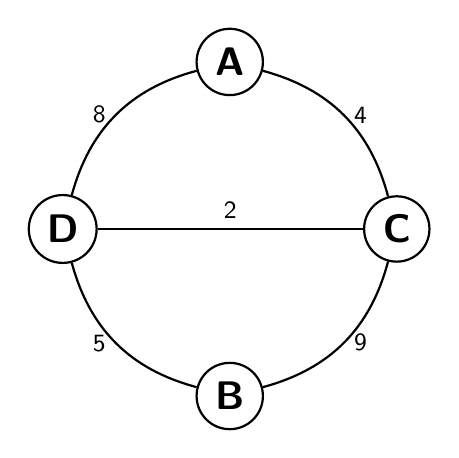
\begin{tikzpicture}[auto, node distance=3cm, every loop/.style={},
		thick,main node/.style={circle,draw,font=\sffamily\Large\bfseries}]
		
		\node[main node] (1) {A};
		\node[main node] (2) [below left of=1] {D};
		\node[main node] (3) [below right of=2] {B};
		\node[main node] (4) [below right of=1] {C};
		
		\path[every node/.style={font=\sffamily\small}]
		(1) edge [bend right] node[left] {8} (2)
		(2) edge node {2} (4)
		edge [bend right] node[left] {5} (3)
		(3) edge [bend right] node[right] {9} (4)
		(4) edge [bend right] node[right] {4} (1);
		\end{tikzpicture}
	\end{center}	
	
	\textit{Solution.} The shortest path from $A \to B$ is the path $P = \left(A, C, D, B\right)$. The weights of every edge included in this path sum to 4 + 2 + 5 = 11, which you will find is the minimum in the set of every path $A \to B$.
	
	\section{Shortest Path Algorithms Survey}
	The following is a list of five algorithms for finding the shortest path between vertices of a graph:
	
	\section{Two Algorithms}
	
	\subsection{Dijkstra's Algorithm}
	Dijksta's
	
	\subsection{Floyd-Warshall Algorithm}
	Floyd Warshall
	
	\section{Comparing Dijkstra's to Floyd-Warshall}
	
	\subsection{Big-O Comparison}
	\tab The time complexities, or Big-O, of these two algorithms can be used to compare their efficiency. The Big-O of Dijkstra's algorithm is $O\left(Vlog\left(V\right)\right)$. The main loop cycles through every unvisited vertex $V$, while the inner loop checks neighbors for that are unvisited. The number of unvisited neighbors goes down as the outer loop continues execution, bringing the inner loop to $log\left(V\right)$.\\
	\tab The Floyd-Warshall algorithm has a time complexity of $O\left(V^{3}\right)$, as a result of the triple nested loop. While this is far worse than Dijkstra's $O\left(Vlog\left(V\right)\right)$, the Floyd-Warshall algorithm solves the all-pairs shortest path problem. This means the shortest path between any pair of vertices can be derived from running the algorithm once. Dijkstra's algorithm would need to be run for every pair of vertices to produce the same results. This would result in a time complexity of $O\left(V^{2}log\left(V\right)\right)$. This narrows the gap between the two algorithms, but ultimately Dijkstra's has a better run time. 
	
	\subsection{Run-time Comparison}
	Run-time Comparison
	
	\begin{thebibliography}{9}
		\bibitem{latexcompanion} 
		Michel Goossens, Frank Mittelbach, and Alexander Samarin. 
		\textit{The \LaTeX\ Companion}. 
		Addison-Wesley, Reading, Massachusetts, 1993.
		
		\bibitem{einstein} 
		Albert Einstein. 
		\textit{Zur Elektrodynamik bewegter K{\"o}rper}. (German) 
		[\textit{On the electrodynamics of moving bodies}]. 
		Annalen der Physik, 322(10):891–921, 1905.
		
		\bibitem{knuthwebsite} 
		Knuth: Computers and Typesetting,
		\\\texttt{http://www-cs-faculty.stanford.edu/\~{}uno/abcde.html}
	\end{thebibliography}
\end{document}
